
\renewcommand{\EntradaBibtex}{AppComidaTamaulipeca_SistemasInteligentes_UPV_2023}


\begin{frame}{\citetitle{\EntradaBibtex} \footnotemark[1] (1)}
\begin{block}{Motivación} 
Desarrollar aplicación enfocada en la comida de una región para obtener información nutricional de la misma
\end{block} 
\begin{itemize}
\item Crear un modelo entrenado (usando TensorFlow) con imágenes de comida (gorditas, flautas, tamales, tortas y pozole)
\item Integar dicho modelo a una aplicación móvil (en Android) 
\item Al tomar una foto con la aplicación, se indique de que alimento se trata, además de su información nutrimental
\end{itemize}
\footnotetext[1]{\fullcite{\EntradaBibtex}}
\end{frame}

\begin{frame}{\citetitle{\EntradaBibtex} (2)}

\begin{center}
	\begin{tabular}{ccccc}
		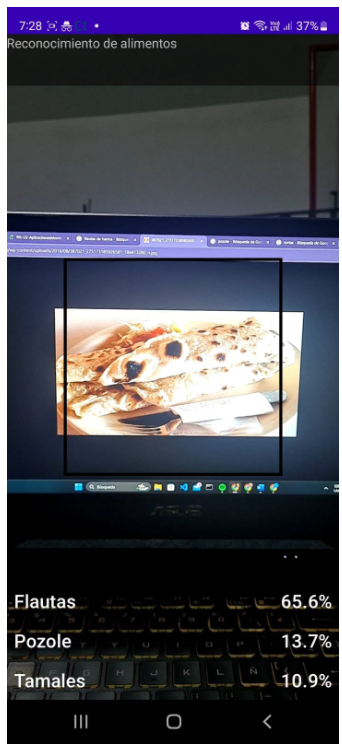
\includegraphics[width=0.18\linewidth,height=4.85cm]{2023_AppComidaTamaulipeca/figs/AppComida1.png} &
		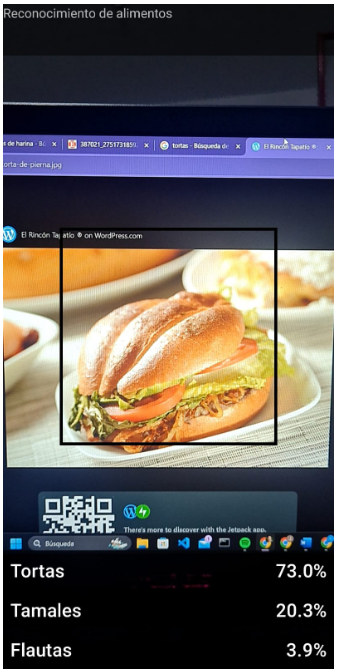
\includegraphics[width=0.18\linewidth,height=4.85cm]{2023_AppComidaTamaulipeca/figs/AppComida2.png} &
		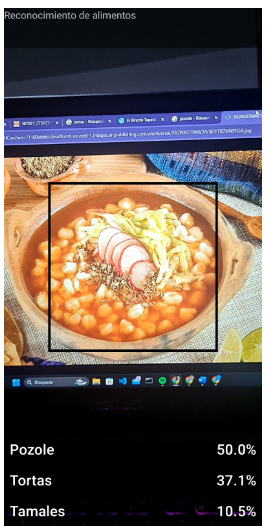
\includegraphics[width=0.18\linewidth,height=4.85cm]{2023_AppComidaTamaulipeca/figs/AppComida3.png} &
		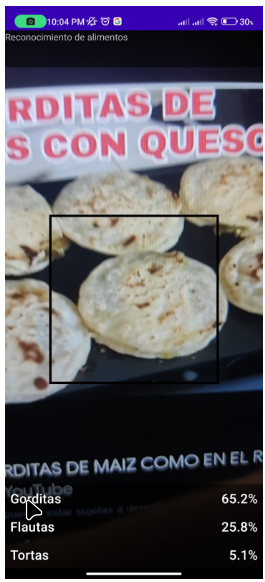
\includegraphics[width=0.18\linewidth,height=4.85cm]{2023_AppComidaTamaulipeca/figs/AppComida4.png} &
		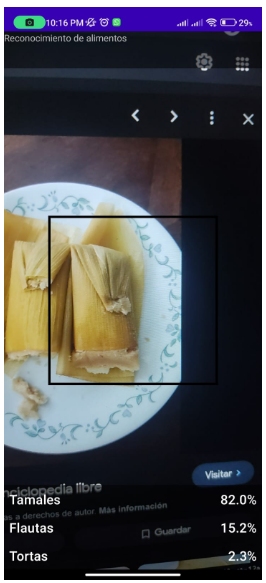
\includegraphics[width=0.18\linewidth,height=4.85cm]{2023_AppComidaTamaulipeca/figs/AppComida5.png}  \\
	\end{tabular}
\end{center}

\end{frame}

%


